% =============================================================
% fig_arch_flatmlp.tex
% Architecture diagram: FlatMLP (spatial-ablation baseline)
% Compile standalone:  pdflatex fig_arch_flatmlp.tex
% =============================================================
\documentclass[tikz, border=8pt]{standalone}
\usepackage{amsmath,amssymb}
\usetikzlibrary{arrows.meta, positioning, fit, backgrounds, calc}

% ---- Shared colour palette (kept identical across all 4 architecture figures) ----
\definecolor{cInput}{HTML}{4477AA}    % blue    - input blocks
\definecolor{cSpatial}{HTML}{8855AA}  % violet  - spatial encoder
\definecolor{cGraph}{HTML}{EE9922}    % amber   - graph components
\definecolor{cTemporal}{HTML}{229988} % teal    - temporal encoder (LSTM)
\definecolor{cOutput}{HTML}{EE6677}   % coral   - output layer
\definecolor{cMuted}{HTML}{999999}    % grey    - "not used in this variant"

% ---- Shared node / arrow styles ----
\tikzset{
  font=\sffamily,
  block/.style={draw=black!70, rounded corners=3pt, line width=0.7pt,
    text width=2.0cm, align=center, font=\sffamily\small,
    minimum height=1.05cm, inner sep=4pt},
  inputblock/.style={block, fill=cInput!15, draw=cInput!75!black, text width=2.4cm},
  spatialblock/.style={block, fill=cSpatial!15, draw=cSpatial!75!black},
  neutralblock/.style={block, fill=black!4, draw=black!55},
  headblock/.style={block, fill=black!4, draw=black!55, text width=2.5cm},
  outputblock/.style={circle, draw=cOutput!75!black, fill=cOutput!25,
    minimum size=1.15cm, font=\sffamily\small, line width=0.7pt},
  mutedblock/.style={block, fill=cMuted!8, draw=cMuted, dashed,
    text=black!55, font=\sffamily\scriptsize\itshape, text width=3.4cm},
  flow/.style={-{Latex[length=2.6mm, width=1.9mm]}, line width=0.9pt, draw=black!70},
  mutedflow/.style={-{Latex[length=2mm, width=1.5mm]}, line width=0.6pt, draw=cMuted, dashed},
  dimlabel/.style={font=\scriptsize\itshape, text=black!60, align=center},
  grouplabel/.style={font=\bfseries\scriptsize, text=black!70, align=center},
  groupbox/.style={draw=black!35, dash pattern=on 3pt off 2pt, rounded corners=4pt, inner sep=8pt},
}

\begin{document}
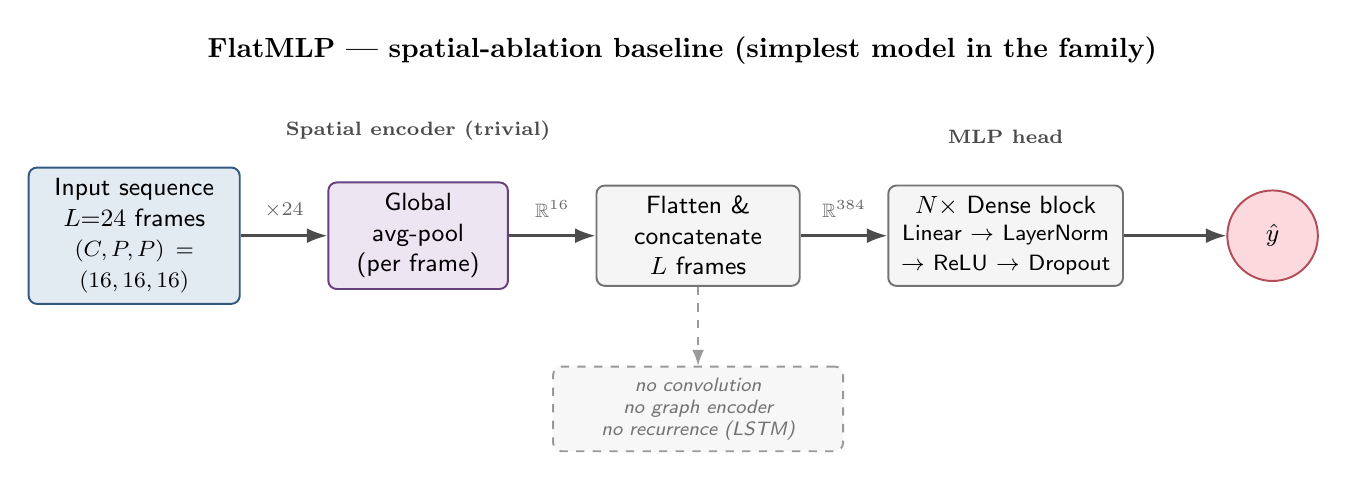
\begin{tikzpicture}[node distance=9mm]

  % ----------------------------------------------------------------
  % Main horizontal flow: input -> pooling -> flatten -> dense -> y
  % ----------------------------------------------------------------
  \node[inputblock] (input)
    {Input sequence\\ $L{=}24$ frames\\ \footnotesize $(C,P,P)=(16,16,16)$};

  \node[spatialblock, right=11mm of input] (pool)
    {Global avg-pool\\ (per frame)};

  \node[neutralblock, right=11mm of pool, text width=2.3cm] (concat)
    {Flatten \&\\ concatenate $L$ frames};

  \node[headblock, right=11mm of concat, text width=2.7cm] (dense)
    {$N\times$ Dense block\\ \footnotesize Linear $\to$ LayerNorm\\ $\to$ ReLU $\to$ Dropout};

  \node[outputblock, right=13mm of dense] (out) {$\hat{y}$};

  % ----------------------------------------------------------------
  % Dimension annotations on the main arrows
  % ----------------------------------------------------------------
  \draw[flow] (input) -- (pool) node[dimlabel, midway, above=1mm] {$\times 24$};
  \draw[flow] (pool) -- (concat) node[dimlabel, midway, above=1mm] {$\mathbb{R}^{16}$};
  \draw[flow] (concat) -- (dense) node[dimlabel, midway, above=1mm] {$\mathbb{R}^{384}$};
  \draw[flow] (dense) -- (out);

  % ----------------------------------------------------------------
  % Skipped components (no conv / graph / recurrence) — drawn muted
  % below the main flow to keep the 4-figure skeleton comparable
  % ----------------------------------------------------------------
  \node[mutedblock, below=10mm of concat] (noop)
    {no convolution\\ no graph encoder\\ no recurrence (LSTM)};
  \draw[mutedflow] (concat.south) -- (noop.north);

  % ----------------------------------------------------------------
  % Group labels above the relevant spans
  % ----------------------------------------------------------------
  \node[grouplabel, above=4mm of pool] {Spatial encoder (trivial)};
  \node[grouplabel, above=4mm of dense] {MLP head};

  % ----------------------------------------------------------------
  % Title / ablation badge
  % ----------------------------------------------------------------
  \node[font=\bfseries\normalsize, above=14mm of concat, xshift=-2mm] (title)
    {FlatMLP --- spatial-ablation baseline (simplest model in the family)};

\end{tikzpicture}
\end{document}
